% !TeX spellcheck = cs_CZ
%{\tikzset{external/prefix={tikz/FYZI/}}
% \tikzset{external/figure name/.add={ch39_}{}}
%=========================== Kapitola: Kinetická teorie plynů =====================================
\setchaptertoc
\chapter{Kinetická teorie plynů}\label{fyz:IchapIXL}  
  \section{Vlastnosti látek}\label{fyz:IchapIXLsecI}
    Touto kapitolou začneme nový předmět, jemuž se budeme poměrně dlouho věnovat. Na začátku našich
    úvah o vlastnostech látek z fyzikálního hlediska si uvědomíme, že látky se skládají z velkého
    množství atomů nebo částic, které na sebe působí elektrickými silami a chovají se podle zákonů
    mechaniky a budeme se snažit pochopit proč se různá seskupení atomů chovají právě určitým
    způsobem.
    
    Je to bezpochyby těžká úloha a snad bude dobré, když si hned na začátku řekneme, že je to
    mimořádně těžký předmět a budeme k němu muset přistupovat jinak, než jsme přistupovali k
    problémům, které jsme řešili do této doby. V případě mechaniky a nauky o světle jsme mohli
    vycházet z přesné formulace některých zákonů jako například Newtonových zákonů nebo vztahu pro
    pole vytvářené urychlovaným nábojem. Pomocí nich jsme mohli vysvětlit mnoho jevů a staly se pro
    nás základem pro chápání mechaniky a optiky. S jejich využitím můžeme ve studiu pokračovat, ale
    už se nenaučíme novou fyziku, jenom se seznámíme s dokonalejšími matematickými metodami řešení
    jednotlivých problémů.
    
    Takový postup však není vhodný ke studiu vlastností látek. O vlastnostech látek můžeme uvažovat
    jen velmi elementárním způsobem. Kdybychom naši analýzu začali základními zákony, kterými jsou
    vlastně zákony mechaniky a elektřiny, byla by příliš složitá. Od těchto zákonů je totiž příliš
    daleko k vlastnostem, které nás zajímají. Je třeba udělat mnoho kroků, než se od Newtonových
    zákonů dostaneme k vlastnostem látek a samotné tyto kroky jsou dost složité. My sice nastoupíme
    tuto cestu a uděláme některé z těchto kroků, ale i když některé z našich analýz budou dost
    přesné, bude tato přesnost postupně ubývat. Získáme tak jen velmi hrubou představu o
    vlastnostech látek.
    
    Jednou z příčin, proč budeme v naší analýze tak nedokonalí, je skutečnost, že vyžaduje hluboké
    vědomosti z teorie pravděpodobnosti. Nebudeme se zajímat o to, jak se každý atom pohybuje, ale
    spíše o to, jaký je střední počet atomů pohybujících se v tom či onom směru a jaké jsou
    pravděpodobnosti různých jevů. Tento předmět si tedy vyžaduje poznání teorie pravděpodobnosti,
    ale naše vědomosti z matematiky nám zatím nestačí a my nechceme své síly přepínat.
    
    Druhou příčinou - z fyzikálního hlediska důležitější - je skutečnost, že atomy se nechovají
    podle klasické mechaniky, ale podle kvantové, takže tento problém správně pochopíme až tehdy,
    když budeme znát kvantovou mechaniku. Na rozdíl od kulečníkových koulí a automobilů je nyní
    rozdíl mezi zákony klasické a kvantové mechaniky velmi důležitý a výrazný, a proto mnohé z věcí,
    jež odvodíme pomocí klasické fyziky, budou principiálně nesprávné. Některé věci nám proto
    zůstanou částečně nepochopené, ale na každou nepřesnost upozorníme, takže budeme vědět, kde
    jsou hranice našeho výkladu. Jedna z příčin, proč jsme v předcházejících kapitolách mluvili o
    kvantové mechanice, spočívá v tom, že musíme vědět, proč je klasická mechanika v některých
    směrech nesprávná.    
    
    Proč se tímto předmětem nyní vůbec zabýváme? Proč půl roku nebo rok nepočkáme, než budeme lépe
    znát teorii pravděpodobnosti a něco z kvantové mechaniky, a tak se jednodušeji dostaneme k
    vlastnostem látek? Proto, že je to těžký předmět a nejlepší způsob, jak se ho naučit, je učit se
    pomalu! Nejprve musíme získat jakousi představu o tom, co by se mělo stát za různých okolností a
    později, když budeme lépe znát základní zákony, zformulujeme vše přesněji.
    
    Kdo by chtěl analyzovat vlastnosti látek v nějakém konkrétním případě, začal by možná tak, že by
    zapsal základní rovnice a pak by se je pokusil matematicky řešit. Existují lidé, kteří se
    pokoušejí postupovat takovým způsobem, ale nejsou úspěšní. Úspěchu dosáhnou ti, kteří začnou
    problém řešit z fyzikálního hlediska, kteří mají hrubou představu o tom, kam směřovat, a pak
    používají správné aproximace, vědí, co je v dané složité situaci malé a co je velké. Tyto
    problémy jsou tak složité, že stojí za to dopracovat se i k jejich elementárnímu chápání, i když
    je nepřesné a neúplné. K takovým problémům se znovu a znovu vracíme a vždy je poznáváme přesněji
    a přesněji, a tak budeme postupovat i v tomto kurzu fyziky.
    
    Další příčina, proč se touto problematikou budeme zabývat už nyní, spočívá v tom, že s mnoha
    takovými myšlenkami jsme se už setkali například v chemii a o některých jste slyšeli už i na
    střední škole. Bude zajímavé poznat fyzikální podstatu těchto věcí.
    
    Jako zajímavý příklad vzpomeňme, že stejné objemy plynů obsahují při stejném tlaku a teplotě
    stejný počet molekul. Zákon násobných poměrů, který říká, že dva plyny, které se slučují v
    chemické reakci, mají objemy v poměru malých celých čísel, pochopil Avogadro jako zákon
    vyjadřující skutečnost, že stejné objemy mají stejné počty atomů. Proč je ve stejných objemech
    stejný počet atomů? Vyplývá něco takového z Newtonových zákonů? Otázkám takového charakteru bude
    věnována tato kapitola. V dalších kapitolách budeme mluvit i o různých jiných jevech
    zahrnujících \textbf{tlak}, \textbf{objem}, \textbf{teplotu} a \textbf{teplo}. 
    
    Zjistíme, že k tomuto předmětu je možné přistupovat nejen z atomistického hlediska, a že
    existuje mnoho vzájemných vztahů mezi vlastnostmi látek. Například, když nějakou látku stlačíme,
    ohřeje se; když ji ohřejeme, zvětší svůj objem. Mezi těmito dvěma skutečnostmi existuje vztah,
    který můžeme odvodit, aniž bychom pochopili vnitřní mechanizmus. Odborná disciplína, jež se
    zabývá takovými vztahy, se nazývá \textbf{termodynamika}. Hluboké pochopení termodynamiky však
    pochází z pochopení vnitřního mechanizmu a tím se právě budeme zabývat. Budeme předpokládat, že
    látky mají atomovou povahu a na základě toho se budeme snažit pochopit jejich různé vlastnosti a
    zákony termodynamiky.
    
    Začneme tedy zkoumat plyny, a to tak, že budeme vycházet z Newtonových zákonů mechaniky.
    
  \section{Tlak plynu}\label{fyz:IchapIXLsecII}
    Víme, že plyn vyvolává \emph{tlak} a naší úlohou bude vysvětlit příčinu tohoto jevu. Kdyby byl
    náš sluch několikrát citlivější, slyšeli bychom stálý rušivý šum. V průběhu vývoje však ucho
    nedosáhlo takové citlivosti, protože by to bylo zbytečné - slyšeli bychom totiž stálý hluk.
    Příčina spočívá v tom, že ušní bubínek je ve styku se vzduchem a vzduch je ohromné množství
    neustále se pohybujících molekul, které na ušní bubínek narážejí. Tyto nárazy molekul vytvářejí
    jakési nepravidelné bubnování, ale my ho neslyšíme, neboť atomy jsou příliš malé a naše ucho
    není dostatečně citlivé. Výsledkem takového neustálého bombardování by mělo být odtlačení
    bubínku, ale protože i na jeho opačné straně dochází k takovému bombardování, je výsledná síla
    nulová. Kdybychom z jedné strany odstranili vzduch nebo kdybychom změnili relativní množství
    vzduchu na stranách bubínku, došlo by k posunutí bubínku na jednu nebo na druhou stranu, protože
    bombardování z jedné strany by bylo větší než bombardování z druhé strany. Tento nepříjemný jev
    pociťujeme tehdy, když stoupáme příliš rychle výtahem nebo letadlem a hlavně, když máme silnou
    rýmu (při rýmě dojde k ucpání trubice, která spojuje vzduch uvnitř bubínku s dutinou ústní s
    vnějším vzduchem a jejich tlaky se nemohou vyrovnat).

    \begin{figure}[ht!] %\ref{fyz:fig242}
      \centering
      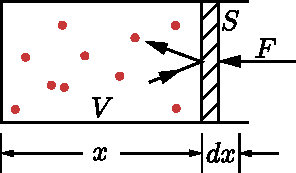
\includegraphics[width=0.7\linewidth]{fyz_fig242.pdf}
      \caption{Atomy plynu v nádobě s pístem, jež se pohybuje bez tření (\cite[s.~525]{Feynman01})}
      \label{fyz:fig242}
    \end{figure}

    Abychom mohli kvantitativně analyzovat tuto situaci, představme si, že se plyn nachází v nádobě
    a na jedné straně nádoby je pohyblivý píst (obr. \ref{fyz:fig242}). Zajímá nás, jaká síla působí
    na píst v důsledku toho, že v nádobě jsou atomy. Atomy se pohybují v nádobě s objemem \(V\)
    všemi možnými rychlostmi a narážejí na píst. Předpokládejme, že na druhé straně pístu není nic,
    jen vakuum. Co se bude dít? Kdyby byl píst ponechán sám sobě a nikdo by ho nepřidržoval, po
    nárazu atomu by vždy získal nepatrnou hybnost a postupně by se vysouval ven z nádoby. Kdybychom
    chtěli zabránit jeho vysouvání, museli bychom ho přidržovat silou \(F\). Zajímá nás, jak velká
    je tato síla. Jeden ze způsobů jak vyjádřit sílu, je udat její velikost připadající na
    jednotkovou plochu. Je-li \(A\) plocha pístu, pak sílu působící na píst můžeme zapsat jako
    součin nějakého čísla a plochy. Tímto způsobem definujeme \textbf{tlak} jako sílu působící na
    píst dělenou plochou pístu
    \begin{mdframed}[style=mdeq] 
      \begin{equation}\label{fyz:eq613}
        p = \frac{F}{S}.
      \end{equation}
    \end{mdframed}

    Abychom lépe pochopili tuto myšlenku (později ji použijeme i k jinému účelu), stanovme
    infinitezimální práci \(\dif W\) konanou při stlačení plynu pístem, který se posunul o
    infinitezimální vzdálenost - \(\dif x\). Tato práce bude rovna součinu síly a posunutí, takže
    podle vztahu (\ref{fyz:eq613}) součinu tlaku, plochy a posunutí. To je záporně vzatý součin
    tlaku a změny objemu
    \begin{equation}\label{fyz:eq680}
      dW=F(−\dif x)= −pS\dif x=−p\dif V.
    \end{equation}

    (Součin plochy \(S\) a vzdáleností \(\dif x\) je změna objemu.) \emph{Záporné znaménko označuje
    skutečnost, že při stlačování se objem zmenšuje; taková volba znaménka vede k tomu, že ke
    stlačení plynu je třeba vykonat práci.}

    Jakou silou musíme tlačit na píst, abychom vykompenzovali nárazy molekul? Píst získává při každé
    srážce hybnost. Každou sekundu dostává píst určitou hybnost a začíná se pohybovat. Abychom
    tomuto pohybu zabránili, musí naše síla odevzdat pístu za sekundu stejně velkou hybnost opačného
    směru. Síla představuje hybnost odevzdanou pístu za sekundu. Můžeme to říci i jinak: Když pístu
    nebudeme bránit v pohybu, získá v důsledku nárazu molekul rychlost; každá další srážka
    představuje malý přírůstek rychlosti, takže píst se bude pohybovat se zrychlením. Zrychlení
    pístu je úměrné síle, jež na něj působí. Síla, o níž jsme říkali, že je \emph{součinem tlaku a
    plochy, je tedy rovna hybnosti odevzdané za sekundu pístu narážejícími molekulami}. Vypočítat
    hybnost za sekundu je snadné - můžeme to udělat ve dvou krocích: Nejprve najdeme hybnost, kterou
    pístu odevzdá při srážce jeden atom a pak tuto hybnost musíme násobit počtem srážek atomu s
    pístem za sekundu. Síla bude právě součin těchto dvou faktorů. Všimneme si těchto dvou faktorů
    blíže. Především předpokládáme, že píst je dokonalým „odrážečem“ atomů. Kdyby nebyl, celá teorie
    by byla chybná, neboť píst by se začal ohřívat a situace by se změnila. Kdyby se však nakonec
    dosáhlo rovnováhy, výsledek by byl takový, že srážky by byly efektivně pružné. V průměru by si
    každá dopadající částice zachovala svou energii. Můžeme si proto představit, že plyn je v
    ustáleném stavu a pístu neodevzdáme žádnou energii, protože píst je v klidu. Když za těchto
    podmínek dopadá částice s určitou rychlostí, odráží se stejnou rychlostí a ovšem se stejnou
    hmotností.

    Je-li \(v\) rychlost atomu a \(v_x\) velikost \(x\)-ové složky \(v\), bude \(mv_x\) velikost
    složky hybnosti ve směru \(x\). Protože tato složka při odrazu od pístu změní směr na opačný a
    zachová si svou velikost, bude celková hybnost dodaná pístu částicí při jedné srážce rovna
    \(2mv_x\).

    Nyní potřebujeme zjistit počet srážek atomů s pístem za sekundu nebo za určitý časový interval
    \(\dif t\) a pak ho dělit intervalem \(\dif t\). Kolik atomů naráží na píst? Předpokládejme, že
    v objemu \(V\) se nachází \(N\) atomů, tedy \(n = N/V\) v každém jednotkovém objemu. Abychom
    určili, kolik atomů narazí na píst, musíme si uvědomit, že za dobu \(t\) nedosáhnou pístu
    všechny částice, které se proti němu pohybují určitou rychlostí, ale jen ty, které jsou dost
    blízko. Jsou-li příliš daleko, projdou za dobu \(t\) jen část cesty k pístu, ale nedosáhnou ho.
    Je jasné, že za dobu \(t\) narazí na píst jen ty částice, které od něho nebudou ve větší
    vzdálenosti než \(v_xt\). Proto je počet srážek za čas \(t\) roven počtu atomů nacházejících se
    ve vzdálenosti ne větší než \(v_xt\) a je-li plocha pístu \(S\), budou atomy, jež narazí na
    píst, zaujímat \emph{objem} \(v_xtS\). Počet atomů, jež narazí na píst, získáme násobením tohoto
    objemu počtem atomů nacházejících se v jednotkovém objemu tedy \(nv_xtS\). My však nechceme
    počet atomů, které narazí za dobu \(t\); zajímá nás počet atomů, které narazí za sekundu a ten
    získáme vydělením tohoto výrazu časem \(t\), dostaneme tedy \(nv_xS\). (Dobu \(t\) můžeme zvolit
    velmi malou, pro eleganci ji můžeme označit \(\dif t\) a pak derivovat. Ale to je vlastně totéž,
    co jsme dělali.)

    Pro sílu tak dostáváme vztah
    \begin{equation}\label{fyz:eq614}
      F=nv_xS\cdot2mv_x.
    \end{equation}
    Všimněte si, že síla je úměrná ploše, je-li při změně plochy hustota částic stálá. Pro tlak
    potom platí vztah
    \begin{equation}\label{fyz:eq615}
      p=2nmv^2_x.
    \end{equation}
   
    Nyní si všimneme některých těžkostí, jež vznikají při takové analýze. Především ne každý atom má
    stejnou rychlost a ne každý se pohybuje týmž směrem. Veličiny \(v_x^2\) jsou tedy pro každý atom
    různé! Každý atom přispívá jinak, a proto musíme vzít \textbf{střední hodnotu} z \(v_x^2\).
    Musíme vzít druhou mocninu z \(v_x\) a zprůměrovat ji přes všechny atomy:
    \begin{equation}\label{fyz:eq616}
      p=nm\langle v^2_x\rangle.
    \end{equation}

    Nezapomněli jsme na koeficient 2? Ne, neboť ze všech atomů směřuje k pístu jen polovina. Ta
    druhá polovina se pohybuje na opačnou stranu, a když bereme \(\langle v^2_x\rangle\),
    průměrujeme druhé mocniny \emph{záporných} i \emph{kladných} \(v_x\). Vezmeme-li tedy prostě
    \(\langle v^2_x\rangle\) a nerozlišujeme kladné a záporné \(v_x\), dostaneme dvakrát tolik, než
    kolik potřebujeme. Střední hodnota z \(v_x^2\), je pro kladná \(v_x\) rovna polovině střední
    hodnoty z \(v_x^2\) pro všechna \(v_x\).

    „Směr osy \(x\)“ není nijak zvlášť charakteristický a atomy narážejí stejně i v ostatních
    směrech. Atomy se stejně dobře pohybují nahoru i dolů, dopředu i dozadu, dovnitř i ven. Proto
    \(\langle v^2_x\rangle\) bude rovna odpovídajícím středním hodnotám v ostatních dvou směrech,
    tedy
    \begin{equation}\label{fyz:eq617}
      \langle v^2_x \rangle = \langle v^2_y \rangle = \langle v^2_z\rangle.
    \end{equation}

    Použitím jednoduchého matematického triku bychom zjistili, že tyto střední hodnoty jsou rovny
    třetině jejich součtu, což je samozřejmě střední hodnota druhé mocniny z rychlosti
    \begin{equation}\label{fyz:eq618}
      \langle v^2_x\rangle = \frac{1}{3}\langle v^2_x+v^2_y+v^2_z\rangle 
                          = \frac{\langle v^2\rangle}{3}
    \end{equation}

    Výhodou takového zápisu je, že se nemusíme starat o nějaký speciální směr a naše formule pro
    tlak získá tvar
    \begin{equation}\label{fyz:eq619}
      p = \frac{2}{3}n\left\langle\frac{mv^2}{2}\right\rangle.
    \end{equation}

    Poslední činitel zapisujeme ve tvaru \(\left\langle\frac{mv^2}{2}\right\rangle\) proto, že
    taková je kinetická energie pohybu těžiště molekuly. Tak jsme vlastně dospěli k vztahu
    \begin{equation}\label{fyz:eq620}
      pV = N\frac{2}{3}\left\langle\frac{mv^2}{2}\right\rangle.
    \end{equation}
    Budeme-li znát rychlosti molekul, můžeme pomocí této rovnice vypočítat tlak.

    Jako jednoduchý příklad uveďme takové plyny jako je helium, argon, rtuťové páry nebo draslíkové
    páry při dost vysoké teplotě, které jsou jednoatomovými plyny a můžeme o nich předpokládat, že
    nemají vnitřní stupně volnosti. Kdybychom měli složitou molekulu, mohl by v ní existovat vnitřní
    pohyb, různé kmity apod. Předpokládejme, že to vše můžeme ignorovat - ve skutečnosti je to vážný
    problém a budeme se k němu muset vrátit, ale v našem případě je takové zanedbání možné. Budeme
    tedy předpokládat, že není třeba uvažovat vnitřní pohyb atomů, a proto pro náš účel kinetická
    energie pohybu molekuly jako celku představuje úplnou energii. V případě jednoatomového plynu je
    kinetická energie celkovou energií. Obecně budeme celkovou energii označovat symbolem \(U\)
    (někdy se nazývá i celkovou vnitřní energií - kdoví proč, vždyť plyn nemá vnější energii), tj.
    půjde o celkovou energii všech molekul plynu nebo jakéhokoliv jiného objektu.

    V případě jednoatomového plynu budeme předpokládat, že celková energie \(U\) je rovna součinu
    počtu atomů a střední kinetické energii každého z nich, neboť neuvažujeme možnost excitace nebo
    vnitřního pohybu atomů. Za těchto okolností můžeme psát
    \begin{equation}\label{fyz:eq621}
      pV = \frac{2}{3}U.
    \end{equation}

    Mimochodem, zde se můžeme na chvíli zastavit a zodpovědět následující otázku: Předpokládejme, že
    máme určité množství plynu a ten pomalu stlačujeme; jaký tlak potřebujeme ke stlačení tohoto
    plynu na určitý objem? je to možno snadno určit, neboť tlak představuje \num{2/3} z energie
    dělené objemem. Při stlačování plynu konáme práci a zvětšujeme energii \(U\). Dostaneme proto
    jakousi diferenciální rovnici: Začneme-li za určitých podmínek, s určitou energií a určitým
    objemem, známe tlak. Začneme-li plyn stlačovat, energie \(U\) poroste a objem \(V\) se bude
    zmenšovat a nás zajímá, jak vzrostl tlak.

    K tomu musíme vyřešit diferenciální rovnici a ihned to provedeme. Je však třeba zdůraznit, že
    předpokládáme, že při stlačování plynu jde všechna práce na zvětšení energie atomů plynu. Můžeme
    se zeptat: \uv{Je vůbec nutné o tom mluvit? Vždyť kam jinam by mohla práce přejít?} Ukazuje se
    však, že práce by mohla přejít i jinam. Existuje tzv. únik tepla stěnami. Horké (tj. rychle se
    pohybující) atomy narážejí na stěny a ohřívají je a tak uniká energie. Zatím budeme
    předpokládat, že k takovým procesům nedochází.

    Náš postup trochu zobecníme, i když stále půjde jen o velmi speciální případ, a místo \(pV=
    \frac{2}{3}U\) budeme psát
    \begin{equation}\label{fyz:eq622}
      pV=(γ−1)U.
    \end{equation}

    Koeficientem \((γ−1)\) násobíme \(U\) proto, protože v budoucnosti budeme pracovat s případy, kdy
    před \(U\) nebudou \num{2/3}, ale nějaké jiné číslo. Označení \((γ−1)\) zvolíme proto, protože
    už téměř sto let používají takové označení fyzici. V našem případě, pro jednoatomový plyn, jako
    například hélium, je \(y\) rovno \num{5/3}, protože tehdy platí \((γ−1) = \num{2/3}\).

    Už jsme si všimli, že při stlačení plynu se koná práce \(-p\dif V\). Stlačení, při němž se
    nedodává a neodvádí tepelná energie, se nazývá \textbf{adiabatické stlačení}. Slovo adiabatický
    pochází z řečtiny: a (ne) + dia (přes) + bainein (jít). (To slovo se používá ve fyzice v různých
    významech a někdy je dost těžké říct, co mají společné.) Při adiabatickém stlačení přechází
    všechna vynaložená práce na změnu vnitřní energie. Podstata tedy spočívá v tom, že nedochází k
    jiným ztrátám energie, a proto máme \(p\dif V = -\dif U\). Platí-li však \(U=pV/(γ−1)\), můžeme
    psát
    \begin{equation}\label{fyz:eq623}
      \dif U = \frac{(p\dif V + V\dif p)}{(γ−1)}.
    \end{equation}
    Máme tedy \(P\dif V= \frac{(p\dif V + V\dif p)}{(γ−1)}\) nebo po přeskupení členů \(γp\dif
    V=−V\dif p\), tedy
    \begin{equation}\label{fyz:eq624}
      \left(\frac{γ\dif V}{V}\right)+\left(\frac{\dif p}{p}\right)=0.
    \end{equation}
    Předpokládáme-li, že \(γ\) je konstanta, což je v případech jednoatomových plynů naštěstí
    oprávněné, můžeme tuto rovnici integrovat a dostaneme \(γ\ln{V}+\ln{P}=\ln{C}\), kde \(\ln{C}\)
    je integrační konstanta. Přejdeme-li k exponenciálám, dostaneme zákon. 
    \begin{equation}\label{fyz:eq625}
      pV^γ=C\qquad \text{(a constant)}.
    \end{equation}
    
    Tento zákon říká, že v adiabatických podmínkách, když se teplo neodvádí a teplota při stlačení
    vzrůstá, je součin tlaku a \num{5/3} mocniny objemu pro jednoatomový plyn konstantní. Ačkoli
    jsme tento zákon odvodili teoreticky, experimenty potvrzují, že jednoatomové plyny se opravdu
    tak chovají.

  \section{Stlačitelnost záření}\label{fyz:IchapIXLsecIII}
    Uvedeme ještě příklad z kinetické teorie plynů, který se v chemii často nepoužívá, ale setkáme
    se s ním v astronomii. Mějme v nádobě ohřáté na velmi vysokou teplotu velký počet fotonů. (Musí
    to být plyn nějaké velmi horké hvězdy. Slunce nemá z tohoto hlediska dost vysokou teplotu; je v
    něm příliš mnoho atomů. Hvězdy mají také mnoho atomů, ale kdyby šlo o velmi horkou hvězdu, bylo
    by možné atomy zanedbat a předpokládat, že máme pouze fotony.) Foton má určitou hybnost
    \(\vr{p}\). (V kinetické teorii máme vždy problém s označováním: \(p\) je tlak, ale \(p\) je
    hybnost; \(V\) je objem, ale \(v\) je rychlost; \(T\) je teplota, ale je to i kinetická energie
    nebo čas nebo moment síly a na to je třeba dávat pozor!) Nyní představuje symbol \(\vr{p}\)
    vektorovou veličinu - hybnost. Analýzu provedeme stejně jako předtím. Za nárazy fotonů bude
    zodpovědná \(x\)-ová složka vektoru \(\vr{p}\)  a dvojnásobek vektoru \(\vr{p}\)  představuje
    hybnost odevzdanou při srážce. Místo \(2mv_x\) máme tedy \(2p_x\) a při výpočtu počtu srážek je
    třeba dosadit tak jako předtím \(v_x\). Takovým způsobem nakonec dostaneme jiné vyjádření vztahu
    (\ref{fyz:eq615}) pro tlak
    \begin{equation}\label{fyz:eq626}
      p = 2np_xv_x.
    \end{equation}
    Po zprůměrování dostaneme \(n\)-násobek střední hodnoty \(p_xv_x\) (o koeficientu 2 jsme již
    mluvili) uvážíme-li i další dva směry, dostaneme
    \begin{equation}\label{fyz:eq681}
      pV=N\langle \frac{\vr{p}\cdot\vr{v}\rangle}{3}.
    \end{equation}  
    To souhlasí se vztahem (\ref{fyz:eq620}), neboť hybnost je rovna \(mv\); je to jen trochu
    obecnější vztah. Součin tlaku a objemu je roven celkovému počtu atomů násobenému střední
    hodnotou z \(\frac{1}{3}(\vr{p}\cdot\vr{v})\).

    Čemu je rovno \(\vr{p}\cdot\vr{v}\) v případě fotonů? Hybnost a rychlost mají stejný směr a
    rychlost je rovna rychlosti světla, takže jde o hybnost fotonu násobenou rychlostí světla.
    Součin hybnosti a rychlosti světla představuje u každého fotonu jeho energii: \(E= pc\) takže
    tyto výrazy jsou energie jednotlivých fotonů a my musíme vzít střední hodnotu energie násobenou
    počtem fotonů. Dostaneme tak \num{1/3} vnitřní energie plynu
    \begin{equation}\label{fyz:eq627}
      pV=\frac{U}{3}\qquad \text{(fotonového plynu)}.
    \end{equation} 
    Stojí-li před \(U\) faktor \num{1/3}, bude v případě fotonů \((γ−1)\) ze vztahu
    (\ref{fyz:eq622}) rovno \num{1/3}, takže \(γ=\num{4/3}\), a proto musí záření v nádobě vyhovovat
    vztahu
    \begin{equation}\label{fyz:eq628}
      pV^{\frac{4}{3}}=C.
    \end{equation}
    Tak jsme se dozvěděli, jaká je stlačitelnost záření! Tento vztah se používá, když se zajímáme o
    to, jak ve hvězdě přispívá záření k tlaku. Nyní vidíme, jak se tento příspěvek počítá a jak se
    mění při stlačení hvězdy. jaké úžasné věci už dokážeme!

  \section{Teplota a kinetická energie}\label{fyz:IchapIXLsecIV}
    Zatím jsme nepřišli do styku s teplotou; zcela úmyslně jsme se tomuto pojmu vyhýbali. Víme, že
    při stlačení plynu energie molekul vzroste a říkáme, že plyn se přitom ohřívá. Bude třeba
    vysvětlit, jak to souvisí s teplotou. Zajímá nás, co je třeba dělat, aby proces neprobíhal
    adiabaticky, ale aby se uskutečnil při konstantní teplotě. Kdybychom k sobě přiložili dvě nádoby
    s plynem a ponechali je tak dostatečně dlouho, měly by obě nakonec stejnou teplotu, i když
    původně to, co nazýváme teplotou, bylo v nádobách různé. Co to znamená? To, že se dostaly do
    situace, v níž by se octly, kdyby byly dostatečně dlouho ponechány samy sobě! Pod rovností
    teplot rozumíme právě to, že se dosáhl konečného stavu, kdy jsou už objekty dost dlouho ve
    vzájemné interakci.
    \begin{figure}[ht!] %\ref{fyz:fig243}
      \centering
      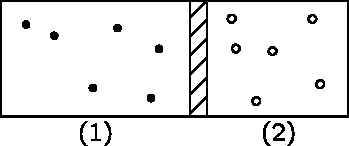
\includegraphics[width=0.7\linewidth]{fyz_fig243.pdf}
      \caption{Atomy dvou různých jednoatomových plynů oddělených pohyblivým pístem
              (\cite[s.~530]{Feynman01})}
      \label{fyz:fig243}
    \end{figure}
    
    Všimněme si, co se stane, když máme dva plyny v nádobě rozdělené pohyblivým pístem (situaci
    znázorňuje obr. \ref{fyz:fig243} a pro jednoduchost předpokládáme, že jde o jednoatomové plyny,
    například helium a neon). V části (1) mají atomy hmotnost \(m_1\), rychlost \(v_1\) a v objemové
    jednotce je jich \(n_1\) a v druhé části mají atomy hmotnost \(m_2\), rychlost \(v_2\) a v
    objemové jednotce je jich \(n_2\). Jaké jsou podmínky rovnováhy?
    
    Je zřejmé, že nárazy zleva způsobují pohyb pístu doprava a stlačování druhého plynu, dokud
    nevzroste jeho tlak a nenastane opačný pohyb pístu, a takový kyvadlový pohyb pístu neustane do
    té doby, dokud se nevyrovnají tlaky na obou stranách. Tak lze zařídit rovnost tlaků; znamená to,
    že vnitřní energie na jednotkový objem jsou si rovny nebo že součin čísla n a střední kinetické
    energie je na obou stranách stejný. My však chceme nakonec ukázat, že i samotné počty \(n_1\) a
    \(n_2\) jsou stejné. Zatím však víme jen to, že součiny takových čísel a kinetických energií
    jsou stejné:    
    \begin{equation*}
      n_1\left\langle\frac{m_1v^2_1}{2}\right\rangle=n_2\left\langle\frac{m_2v^2_2}{2}\right\rangle,
    \end{equation*}
    
    To vyplývá ze vztahu (\ref{fyz:eq619}), neboť tlaky jsou stejné. Musíme si uvědomit, že to z
    dlouhodobého hlediska není jediná podmínka, ale že musí probíhat i nějaký další, pomalejší
    proces, než se ustaví úplná rovnováha se stejnými teplotami.
    
    Abychom lépe pochopili oč jde, předpokládejme, že tlak na levé straně je vyvolán velkou
    hustotou, ale malými rychlostmi atomů. Při velkém \(n\) a malém \(v\) můžeme dosáhnout stejného
    tlaku jako při malém \(n\) a velkém \(v\). Atomy se mohou pohybovat pomalu a být víc nahuštěny
    nebo jich může být méně, ale mohou narážet na píst prudčeji. Zůstane to tak trvale? Na první
    pohled by se zdálo, že ano, ale když se vážně zamyslíme, zjistíme, že jsme zanedbali jednu velmi
    důležitou věc. Neuvědomili jsme si, že přehrazovací píst není vystaven trvalému tlaku, ale
    chvěje se tak jako ušní bubínek, o němž jsme již mluvili. K tomuto chvění dochází proto, že
    nárazy nejsou zcela pravidelné. Nemáme co dělat s konstantním tlakem, ale s jakýmsi vytrvalým
    bubnováním - tlak se neustále mění a proto píst poskakuje. Předpokládejme, že atomy na pravé
    straně narážejí na píst dosti pravidelně, ale atomy na levé straně, i když jejich méně a jejich
    nárazy jsou řidší, mají velkou energii. Proto dostane píst čas od času silný impulz zleva, pohne
    se proti pomalým atomům na pravé straně a zrychlí je. (Při srážce s pístem každý atom získá nebo
    ztratí energii podle toho, na kterou stranu se pohybuje píst při srážce s atomem.) V důsledku
    srážek tedy píst poskakuje a poskakuje a rozechvívá i ostatní plyn - tak odevzdává energii jiným
    atomům a jejích pohyb se zrychluje, dokud nenastane rovnováha. K určité rovnováze dojde tehdy,
    když se píst bude pohybovat takovou střední kvadratickou rychlostí, že bude stejně rychle
    odebírat energii atomům, jako jim odevzdávat. Píst tedy získává jakousi nepravidelnost rychlosti
    a my ji musíme určit. Když se nám to podaří, budeme blíž k vyřešení problému, protože plyny
    budou měnit rychlosti svých atomů do té doby, dokud nenastane taková situace, že každý plyn bude
    prostřednictvím pístu získávat tolik energie, kolik ztrácí.
    
    Je velmi obtížné určit pohyb uvažovaného pístu ve všech jeho detailech. I když se tyto věci
    velmi snadno chápou, dost těžko se analyzují. Dřív, než se do takové analýzy pustíme, všimněme
    si jiného problému. Uvažujme nádobu s plynem, který je tvořen dvěma druhy molekul s hmotnostmi
    \(m_l\) a \(m_2\), rychlostmi \(v_1\) a \(v_2\) atd. Proti předcházejícímu případu máme nyní
    mnohem těsnější kontakt dvou částí. Kdyby molekuly druhého druhu byly v klidu, netrvalo by to
    dlouho, protože by do nich narážely molekuly prvního druhu a udělily by jim rychlost. I kdyby se
    molekuly druhého druhu pohybovaly mnohem rychleji než molekuly prvního druhu, nebyl by tento
    stav trvalý a nakonec by tyto molekuly odevzdaly molekulám prvního druhu část své energie. Naší
    úlohou je najít pravidlo, které by určovalo relativní rychlosti molekul takových dvou plynů
    nacházejících se v jedné nádobě.
    
    I tato úloha je velmi obtížná, ale vyřešíme ji následujícím způsobem. Nejprve se budeme zabývat
    jedním částečným problémem (opět jde o případ, kdy dostaneme snadno zapamatovatelný výsledek,
    ale odvození si vyžaduje hodně důvtipu.) Předpokládejme, že se srazí dvě molekuly, které mají
    různé hmotnosti a že tuto srážku pozorujeme z těžiště těchto dvou molekul, abychom se vyhnuli
    komplikacím. Ze zákonů pružných srážek při zachování celkové hybnosti a energie už víme, že se
    molekuly mohou po srážkách pohybovat pouze tak, že každá si zachová velikost své původní
    rychlosti a změní se jen směr jejich pohybu. Takovou typickou srážku znázorňuje obrázek
    \ref{fyz:fig244}. Na chvíli předpokládejme, že pozorujeme všechny srážky v podmínkách, kdy
    těžiště je v klidu. Dále si představme, že se všechny molekuly pohybují zpočátku horizontálně.
    Po první srážce se samozřejmě některé z molekul odchýlí o určitý úhel. Jinými slovy, i když se
    původně všechny pohybovaly horizontálně, budou se později aspoň některé pohybovat vertikálně. Po
    dalších srážkách se opět změní směr jejich pohybu a budou se pohybovat pod jiným úhlem. I kdyby
    zpočátku byly dokonale organizovány, rozletí se do různých směrů a tak to půjde dále. Ptáme se k
    čemu to nakonec povede. Odpověď je taková: \emph{Každá dvojice atomů se bude se stejnou
    pravděpodobností pohybovat v každém směru prostoru.} Pak už další srážky nemohou změnit
    rozdělení.
    
    \begin{figure}[ht!] %\ref{fyz:fig244}
      \centering
      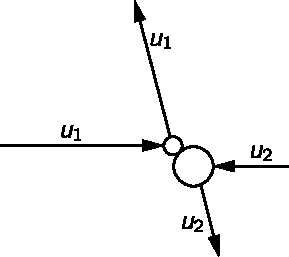
\includegraphics[width=0.6\linewidth]{fyz_fig244.pdf}
      \caption{Srážka dvou různých molekul v těžišťové vztažné soustavě (center-of-mass (CM) system)
              \(u_1=\abs{\vec{v}_1−\vec{v}_{CM}}\), \(u_2=\abs{\vec{v}_2−\vec{v}_{CM}}\)
              (\cite[s.~531]{Feynman01})}
      \label{fyz:fig244}
    \end{figure}
    
    Co máme rozumět tím, že v každém směru se budou molekuly pohybovat se stejnou pravděpodobností?
    \emph{Nemůžeme} samozřejmě mluvit o pravděpodobnosti pohybu v určitém směru, neboť směr je něco
    velmi úzkého a my musíme vztahovat pravděpodobnost k jednotce „něčeho“. Naši myšlenku však
    můžeme vyjádřit tak, že danou částí kulové plochy, která má střed v bodě srážky, prochází stejně
    množství molekul jako kteroukoliv jinou stejně velkou částí této plochy. Výsledek srážek je pak
    takové rozdělení molekul podle směrů, při kterém stejným částem kulové plochy odpovídá stejná
    pravděpodobnost.
    
    Mimochodem, kdybychom porovnávali původní směr se směrem odkloněným o úhel \(\vartheta\), přišli
    bychom na zajímavou vlastnost: elementární ploška na kouli s jednotkovým poloměrem je rovna
    \(2\pi\)-násobku výrazu \(\sin\vartheta\dif\vartheta\), ale to je stejný výraz jako diferenciál
    \(\cos\vartheta\). To znamená, že kosinus úhlu \(\vartheta\) mezi dvěma směry se stejnou
    pravděpodobností nabývá libovolné hodnoty z intervalu od \num{-1} do \num{+1}.

    Nyní musíme věnovat pozornost té skutečnosti, že srážky neprobíhají v těžišťové soustavě, ale
    atomy mají před srážkou rychlosti \(v_1\) a \(v_2\). Srážku s takovými rychlostmi můžeme pak
    analyzovat následujícím způsobem. Těžiště soustavy dvou atomů se pohybuje „střední“ rychlostí s
    váhami úměrnými hmotnostem, takže pro rychlost těžiště \(v_T\) platí: 
    \begin{equation*}
      v_{CM} = \frac{m_1v_1 + m_2v_2}{m_1 + m_2}
    \end{equation*}
    Pozorujeme-li srážku v těžišťové soustavě, vypadá tak, jako na obr. \ref{fyz:fig244}, kdy se
    atomy srážejí určitou relativní rychlostí \(w\). Tou relativní rychlostí je právě \(v_1-v_2\).
    Situace je pak taková, že soustava spojená s těžištěm se pohybuje a v této soustavě se molekuly
    přibližují relativní rychlostí \(w\), srazí se a pohybují se v nových směrech. Zatímco se to
    odehrává, těžiště se pohybuje nerušeně dál.

    Jaké je rozdělení molekul, jež získáme takovým způsobem? Argumenty, které jsme uvedli, vedou k
    závěru: \emph{V rovnováze jsou stejně pravděpodobně všechny směry \(w\) vzhledem ke směru pohybu
    těžiště.\footnote{Taková argumentace, kterou kdysi použil Maxwell, má hlubší pozadí. I když je
    závěr správný, bezprostředně nevyplývá z úvah o symetrii, o které jsme se předtím opírali. Při
    přechodu ke vztažně soustavě pohybující se plynem by mohlo dojit k narušení rozdělení rychlosti.
    Jednoduchý důkaz našeho výsledku se nám nepodařilo najít.}} Mezi směrem relativní rychlosti a
    směrem pohybu těžiště nebude nakonec žádná korelace. I kdyby byla, srážky by ji narušovaly,
    takže by vymizela. Proto je střední hodnota kosinu úhlu mezi \(w\) a \(W_T\) rovna nule. Platí
    tedy
    \begin{equation}\label{fyz:eq629}
      \left\langle\vec{w}\cdot\vec{v}_{CM}\right\rangle = 0
    \end{equation}
    Jenže \(\vec{w}\cdot\vec{v}_{CM}\) můžeme vyjádřit pomocí \(\vec{v}_1\) a \(\vec{v}_2\)
    \begin{align}
      \vec{w}\cdot\vec{v}_{CM} 
        &= \frac{(\vec{v}_1−\vec{v}_2)\cdot(m_1\vec{v}_1+m_2\vec{v}_2)}{m_1+m_2} \nonumber \\
        &= \frac{(m_1v^2_1−m_2v^2_2)+(m_2−m_1)(v_1\cdot v_2)}{m_1+m_2} \label{fyz:eq630}
    \end{align}

    Nejprve si všimněme \(\vec{v}_1\cdot\vec{v}_2\) a zeptejme se, jaká bude střední hodnota
    \(\vec{v}_1\cdot\vec{v}_2\). Zajímáme se tedy o to, jaká bude střední složka rychlosti jedné
    molekuly ve směru pohybu druhé molekuly. Je jasné, že molekula se bude stejně pravděpodobně
    pohybovat na jednu stranu i na stranu k ní opačnou. \emph{Střední hodnota rychlostí
    \(\vec{v}_2\) je v libovolném směru nulová}. Proto je i ve směru \()\vec{v}_1\) střední hodnota
    \(\vec{v}_2\) nulová. Střední hodnota \(\vec{v}_1\cdot\vec{v}_2\) je tedy rovna nule! Tak jsme
    dospěli k tvrzení, že podle (\ref{fyz:eq630}) musí být střední hodnota \(m_1v^2_1\) rovna
    střední hodnotě \(m_2v^2_2\). To ale znamená, že \emph{střední kinetické energie obou molekul
    musí být stejné}
    \begin{equation}\label{fyz:eq631}
      \left\langle\frac{1}{2}m_1v^2_1\right\rangle = \left\langle\frac{1}{2}m_2v^2_2\right\rangle.
    \end{equation}

    Kdyby se plyn skládal ze dvou druhů atomů, bylo by možné ukázat (předpokládáme, že se nám
    to podařilo ukázat), že střední hodnota kinetické energie jednoho druhu atomů je stejná jako
    střední hodnota kinetické energie druhého druhu atomů, pokud se oba druhy atomů nacházejí v
    jedné nádobě a jsou v rovnováze. To znamená, že těžší atomy se pohybují pomaleji než lehčí.
    Snadno se o tom můžeme přesvědčit pomocí experimentu S „atomy“ různých hmotností na vzduchové
    dráze.

    Dále se budeme zajímat o dva různé plyny oddělené v nádobě a ukážeme, že i takové plyny mají po
    dosažení rovnováhy stejné střední hodnoty kinetické energie, a to i tehdy, když nejsou v téže
    části nádoby. Důkaz můžeme provést různými způsoby. Jeden ze způsobů předpokládá pevnou
    přihrádku mezi plyny, v níž je tak nepatrný otvor (obr. \ref{fyz:fig245}), že jím jeden plyn
    může procházet, ale druhý ne, protože má příliš velké molekuly. Nastane-li rovnováha, pak se v
    té části, kde je směs molekul, střední hodnoty energie molekul obou druhů vyrovnají. Menší
    molekuly však procházejí otvorem beze ztráty kinetické energie, takže střední hodnoty kinetické
    energie v čistém plynu a směsi musí být stejné. Tento důkaz není dost uspokojivý, neboť takový
    druh otvoru separující jednotlivé druhy molekul nemusí existovat.

    \begin{figure}[ht!] %\ref{fyz:fig245}
      \centering
      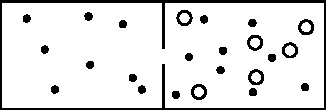
\includegraphics[width=0.7\linewidth]{fyz_fig245.pdf}
      \caption{Dva plyny v nádobě s polopropustnou membránou (\cite[s.~533]{Feynman01})}
      \label{fyz:fig245}
    \end{figure}

    Vraťme se proto k naší úloze s pístem. Můžeme ukázat, že kinetická energie pístu musí být také
    rovna ¨\(\frac{1}{2}m_2v^2_2\). Ve skutečnosti jde o kinetickou energii čistě horizontálního
    pohybu pístu, a proto, když odhlédneme od jeho vertikálního pohybu, dostaneme vlastně
    \(\frac{1}{2}m_2v^2_{2_x}\). Budeme-li vycházet z rovnováhy na druhé straně, můžeme stejným
    způsobem dokázat, že kinetická energie pístu je rovna \(\frac{1}{2}m_1v^2_{1_x}\). I když píst
    není uprostřed plynu, ale na jedné jeho straně, můžeme opět tvrdit, že střední kinetická energie
    pístu a molekul plynu jsou v důsledku srážek stejné, i když takový důkaz je trochu obtížnější.

    Kdyby nás ani takový postup neuspokojil, můžeme si vymyslet příklad, v němž by se zabezpečovala
    rovnováha zařízením, na které naráží molekuly každého plynu ze všech stran. Předpokládejme, že
    máme krátkou tyč, která prochází pístem a na každém konci má kouli. Tato tyč se může pohybovat
    ložiskem v pístu bez tření. Každá z koulí je vlastně jakoby velká molekula a molekuly plynu na
    ni mohou narážet ze všech stran. Celý takový objekt má určitou hmotnost \(m\) a opět máme
    molekuly plynu s hmotnostmi \(m_l\), \(m_2\). Stejnou analýzou srážek jako dříve bychom
    zjistili, že kinetická energie objektu s hmotností \(m\) musí být v důsledku nárazů molekul z
    jedné strany v průměru rovna \(\frac{1}{2}m_1v^2_1\). Podobně v důsledku srážek s molekulami na
    druhé straně musí být střední kinetická energie rovnat \(\frac{1}{2}m_2v^2_2\). Obě strany proto
    musí mít stejnou kinetickou energii, jsou-li v tepelné rovnováze. Výsledek získaný v případě
    směsi plynů lze takovým způsobem zobecnit na případ dvou různých, oddělených plynů při stejné
    teplotě.

    \emph{Máme-li tedy dva plyny se stejnou teplotou, budou střední kinetické energie molekul těchto
    plynů v těžišťové soustavě stejné.}

    Střední kinetická energie molekul je vlastností pouze „teploty“. Protože závisí na „teplotě“, a
    ne na samotném plynu, můžeme ji využít k definování teploty. Střední kinetická energie molekuly
    je tedy určitou funkcí teploty. Jakou stupnici však máme použít k určování teploty? Mohli bychom
    svévolně definovat teplotní stupnici tak, aby střední energie byla přímo úměrná teplotě. Nejlépe
    by bylo udělat to tak, že bychom samotnou střední energii nazvali „teplotou“. To by byla
    nejjednodušší funkce. Bohužel teplotní stupnice byla zvolena jinak a místo toho, abychom střední
    energii nazvali přímo teplotou, používáme konstantní koeficient, který dává do souvislosti
    střední energii molekuly a stupeň absolutní teploty, který nazýváme \textbf{kelvin}. Konstanta
    úměrnosti\footnote{Celsiova stupnice je vlastně Kelvinova stupnice, v níž považujeme za nulu
    \num{273.15} stupně, takže platí: \(T = \num{273.15} +\) Celsiova teplota.} je \(k =
    \SI{1.38e-23}{\joule\per\kelvin}\). Při absolutní teplotě \(T\) je střední kinetická energie
    molekuly rovna \(\frac{3}{2}kT\). (Koeficient \num{3/2} jsme zavedli jen z praktických důvodů,
    abychom se zbavili číselných koeficientů v jiných vztazích.) Je třeba poznamenat, že kinetická
    energie připadající na jednu složku pohybu v kterémkoliv směru je rovna jen \(\frac{1}{2}kT\).
    Tři nezávislé směry pohybu vedou k hodnotě \(\frac{3}{2}kT\).

  \section{Zákon ideálního plynu}\label{fyz:IchapIXLsecV}
    Nyní můžeme aplikovat naši definici teploty v rovnici (\ref{fyz:eq620}) a tak najít zákon
    závislosti tlaku plynu na teplotě, který zní: Součin tlaku a objemu je roven součinu celkového
    počtu atomů, univerzální konstanty \(k\) a teploty \(T\).
    \begin{equation}\label{fyz:eq632}
      \boxed{pV=NkT}.
    \end{equation}

    Navíc při daných hodnotách teploty, tlaku a objemu je počet atomů přesně určen a také
    představuje univerzální konstantu! Stejné objemy různých plynů proto mají při stejném tlaku a
    stejné teplotě stejný počet molekul a to je důsledek Newtonových zákonů. Je to opravdu
    překvapující důsledek!

    V praxi, když máme pracovat s molekulami, musíme používat velmi velká čísla, a proto chemici
    vybrali jedno velmi velké číslo a dali mu speciální název, a to \textbf{mol}. Molem je tedy
    třeba chápat určité praktické číslo. Zůstává historickou otázkou, proč nevybrali kulaté číslo
    např. \num{10e24}. Za počet objektů, který slouží jako standard, bylo vybráno číslo \(N_0 =
    \num{6.02e23}\), a toto číslo dostalo název mol. Místo měření počtu molekul v jednotkách se měří
    tento počet v molech\footnote{To, co chemici nazvali molekulární váhou, je vlastně hmotnost molu
    molekul v gramech. Mol je definován tak, že hmotnost molu atomů izotopu uhlíku 12 (jeho jádra se
    skládají ze 6 protonů a 6 neutronů) je rovna přesně \num{12} gramů.}.  Pomocí \(N_0\) můžeme
    vyjádřit počet molů, násobit ho počtem atomů v molu a dále násobit veličinou \(kT\). Počet atomů
    v molu násobený veličinou \(k\) je vlastně molární hodnota \(k\) a používá se pro ni speciální
    označení \(R\). Molární hodnota \(k\) je rovna \num{8.317} joulu: \(R = N_0k =
    \SI{8.317}{\joule\per\mol\kelvin}\). Zákon ideálního plynu tedy můžeme zapsat ve tvaru
    obsahujícím součin počtu molů (označujeme ho také písmenem \(N\)\footnote{ V češtině se tento
    základní zákon nazývá stavová rovnice Ideálního plynu a zapisuje se ve tvaru \(pV=nRT\), kde
    počet molů (látkové množství) je označeno písmenem \(n\).} a veličiny \(RT\) nebo součin počtu
    atomů a veličiny \(kT\).
    \begin{equation}\label{fyz:eq633}
      \boxed{pV=NRT}.
    \end{equation}

    Je to stejný zákon, ale vyjádřený v jiných jednotkách. My používáme jako jednotku číslo \num{1},
    ale chemici číslo \num{6e23}.

    Ještě se zmíníme o zákonu ideálního plynu v případě, kdy máme co dělat s objekty, jež jsou
    odlišné od jednoatomových molekul. Do této doby jsme se zabývali pohybem atomů jednoatomového
    plynu v soustavě spojené s těžištěm. Ptáme se, co se stane, když se přidají i síly. Nejprve si
    všimneme případu, kdy je píst udržován horizontální pružinou, takže na něj působí síly. Pohyb
    vyvolávající nárazy mezi atomy a pístem nezávisí v žádném časovém okamžiku na tom, kde se právě
    píst nachází. Rovnovážné podmínky zůstávají stejné. Rychlost pohybu pístu bude nezávisle na jeho
    poloze právě taková, aby předával molekulám energii jako dříve. Nezáleží tedy na pružině.
    Rychlost, s níž se musí pohybovat píst, je v průměru stejná. Naše poučka, že střední hodnota
    kinetické energie vjednom směruje rovna \(\frac{1}{2}kT\), \emph{zůstává v platností bez ohledu na to
    zda působí či nepůsobí síly}.

    Uvažujme jako příklad dvouatomovou molekulu složenou z atomů o hmotnostech \(m_A\) a \(m_B\).
    Dokázali jsme, že pohyb částí \(A\) a \(B\) v těžišťové soustavě je takový, že
    \(\left\langle\frac{1}{2}m_Av^2_A\right\rangle=\left\langle\frac{1}{2}m_Bv^2_B\right\rangle =
    \frac{3}{2}kT\). Jak je to ale možné, když jsou tyto části vzájemně spojeny? I když jsou
    spojeny, výměna energie při vzájemné rotaci a vibraci, při srážkách s jinými molekulami závisí
    pouze na tom, jak rychle se pohybují. Právě to určuje rychlost výměny energie při srážkách. V
    daném časovém okamžiku není síla rozhodující. Proto platí stejný princip i tehdy, působí-li
    síly.

    Nakonec bychom měli dokázat, že zákon ideálního plynuje správný i tehdy, zanedbáme-li vnitřní
    pohyb molekul. Do této doby jsme vlastně s vnitřním pohybem nepočítali, protože jsme zkoumali
    jednoatomový plyn. Nyní však ukážeme, že rychlost těžiště libovolného objektu, který můžeme
    považovat za těleso o hmotnosti \(M\), je taková, že platí
    \begin{equation}\label{fyz:eq634}
      \left\langle\frac{1}{2}Mv^2_{CM}\right\rangle = \frac{3}{2}kT.
    \end{equation}
    Jinak řečeno, můžeme sledovat buď jednotlivé části nebo těleso jako celek! Podívejme se, proč
    tomu tak je: Hmotnost dvouatomové molekul je \(M = m_A + m_B\) a pro rychlost těžiště \(v_{CM}\)
    platí \(v_{CM} = (m_Av_A + m_Bv_B)/M\). Potřebujeme znát \(⟨v^2_{CM}⟩\). Umocníme-li \(v_{CM}\),
    dostaneme
    \begin{equation}\label{fyz:eq635}
      v^2_{CM} = \frac{m^2_Av^2_A+2m_Am_B(\vec{v}_A\cdot\vec{v}_B)+m^2_Bv^2_B}{M^2}
    \end{equation}
    Násobíme-li tento výraz veličinou \(\frac{1}{2}M\) a najdeme střední hodnotu pro
    \(\left\langle\frac{1}{2}Mv^2_{CM}\right\rangle\), dostaneme
    \begin{align}
      &= \frac{m_A\frac{3}{2}kT + m_Am_B⟨\vec{v}_A\cdot\vec{v}_B⟩ + m_B\frac{3}{2}kT}{M}\nonumber\\
      &= \frac{3}{2}kT + \frac{m_Am_B⟨\vec{v}_A\cdot\vec{v}_B⟩}{M}                \label{fyz:eq636}
    \end{align}
    (Využili jsme skutečnost, že \((m_A + m_B)/M=1\).) Čemu je rovna  \(⟨\vec{v}_A\cdot\vec{v}_B⟩\)?
    (Nejlepší by bylo, kdyby byla rovna 0!) Abychom to zjistili, použijeme náš předpoklad, že
    relativní rychlost \(\vec{w} = \vec{v}_A-\vec{v}_B\) má v každém směru stejnou pravděpodobnost,
    takže střední hodnota její složky do kteréhokoliv směru je rovna nule. Budeme tedy předpokládat,
    že
    \begin{equation}\label{fyz:eq638}
      ⟨\vec{w}\cdot\vec{v}_{CM}⟩=0.
    \end{equation}
    Co však představuje \(\vec{w}\cdot\vec{v}_{CM}\)? Je to
    \begin{align}
        &= \frac{(\vec{v}_A−\vec{v}_B)⋅(m_A\vec{v}_A+m_B\vec{v}_B)}{M}                   \nonumber\\
        &= \frac{m_Av^2_A+(m_B−m_A)(\vec{v}_A\cdot\vec{v}_B)−m_Bv^2_B}{M}          \label{fyz:eq637}
    \end{align}
    Protože \(⟨m_Av^2_A⟩=⟨m_Bv^2_B⟩\), vyruší se ve střední hodnotě první a poslední člen a zůstane
    nám
    \begin{equation}\label{fyz:eq639}
      (m_B−m_A)⟨\vec{v}_A\cdot\vec{v}_B⟩=0.
    \end{equation}
    Je-li \(m_A≠m_B\), bude \(⟨\vec{v}_A\cdot\vec{v}_B⟩=0\), a proto pohyb celé molekuly jako tělesa
    o hmotnosti \(M\) má kinetickou energii, v průměru rovnou \(\frac{3}{2}kT\).

    Současně jsme ukázali, že střední kinetická energie \emph{vnítřního} pohybu dvouatomové
    molekuly, neuvažujeme-li pohyb těžiště, je rovna \(\frac{3}{2}kT\). Vždyť celková kinetická
    energie částí molekuly je \(\frac{1}{2}m_Av^2_A+\frac{1}{2}m_Bv^2_B\) a její střední hodnota je
    rovna \(\frac{3}{2}kT + \frac{3}{2}kT\), tedy \(3kT\). Kinetická energie pohybu těžiště je rovna
    \(\frac{3}{2}kT\), a proto střední kinetická energie rotačního a vibračního pohybu dvou atomů v
    molekule, kterou dostaneme z rozdílu těchto energií, musí být rovna \(\frac{3}{2}kT\).

    Věta o střední energii pohybu těžiště má obecný charakter: V případě libovolného objektu, který
    zkoumáme jako celek v přítomnosti nebo nepřítomnosti sil, je střední kinetická energie každého
    nezávislého pohybu rovna \(\frac{1}{2}kT\). Takové „nezávislé směry pohybu“ nazýváme
    \emph{stupně volnosti systému}. Počet stupňů volnosti molekuly složené z \(r\) atomů je roven
    \(3r\), neboť k určení polohy každého atomu potřebujeme tři souřadnice. Celkovou kinetickou
    energii molekuly lze vyjádřit bud' jako součet kinetických energií jednotlivých atomů nebo jako
    součet kinetické energie pohybu těžiště a kinetické energie vnitřního pohybu. Vnitřní pohyb je
    někdy možné vyjádřit jako součet rotační a vibrační energie molekuly, ale takové vyjádření je
    jen určitou aproximací. Aplikujeme-li naše tvrzení na \(r\)-atomovou molekulu, zjistíme, že
    molekula má v průměru \(\frac{3rkT}{2}\) joulů kinetické energie, z čehož \(\frac{3}{2}kT\)
    joulů připadá na kinetickou energii těžiště celé molekuly a zbytek, tj. \(\frac{3}{2}(r-1)kT\)
    Joulů, připadá na vnitřní vibrační a rotační kinetickou energii.

  \section{Příklady a cvičení}\label{fyz:IchapIXLsecVI}

%} %tikzset
%---------------------------------------------------------------------------------------------------